% --------------------------------------------------------------------

\section{Introduction}

In the past fifteen years, 
there have been rapid advances in the algorithms for combinatorial problems. 
This has been greatly sparked by the development in algebraic techniques for solving the 
multilinear monomial detection problem, that is, 
deciding whether a multivariate (multiple variables) 
polynomial contains a multilinear monomial\footnote{ 
i.e., a term of multiple variables where each variable appears at most once. 
See also Section \ref{sect:prelims_algebra}}. 
\amnote{I do see this style of footnotes from time to time, but some people are
not fond of it. Parentheses might be a better choice.}
Multilinear monomial detection for parameterized combinatorial problems was 
first introduced by \citeauthor{Koutis05} in an early work 
\cite{Koutis05}, where a set packing problem is 
reduced to multilinear monomial detection.

\amnote[inline,nomargin]{(Namely,)} the technique of \emph{algebraic fingeprinting},   
introduced by \citeauthor{Koutis08} \cite{Koutis08} and further developed by 
\citeauthor{Williams09} \cite{Williams09}, 
has found great success for many combinatorial problems. 
For instance with algebraic fingerprinting, the $k$-path problem 
that previously could be solved in
\amnote*{Move footnote elsewhere}{\bigOstar{4^{k}}}
\footnote{$\mathcal{O}$* may hide factors polynomial to input size. 
See Section \ref{sect:prelims_other}} 
time by \citeauthor{Chen07} \cite{Chen07}, 
\amnote*[inline,nomargin]{can now}{could be} solved in \bigOstar{2^{3k/2}} time \cite{Koutis08}. 
This result was quickly improved by \textcite{Williams09}, %\cite{Williams09}, 
\amnote{Tip: use \texttt{\textbackslash textcite} and friends}
who gave an \bigOstar{2^k} algorithm.

Most famously, 
\citeauthor{Björklund14} \cite{Björklund14} published an algorithm 
that solved the famous Hamiltonian problem (Hamiltonicity) in \bigOstar{1.657^n} time 
with clever utilizations of this novel algebraic technique. 
The fastest algorithms for Hamiltonicity before this ran in \bigOstar{2^n} time
\amnote*[inline,nomargin]{and date from \citeyear{HelKar62}}{%
, and were known since 1962
}
\cite{HelKar62}, \cite{Bellman62}. 
This was a significant improvement on a problem 
that had seen no progress in nearly fifty years! 
Soon
\amnote*[inline,nomargin]{thereafter, a \bigOstar{1.657^k} algorithm was found
for the related (?) $k$-path problem}{
enough for $k$-path, 
an \bigOstar{1.657^k} algorithm was found
} \cite{Björklund17}.

\subsection{Research scope and thesis structure}

The goals of this bachelor's thesis are 
to find out how multilinear monomial detection is relevant in combinatorial problems, 
and how algebraic fingerprints can be utilized to design faster 
algorithms for these problems. For the reader with background in computer science, 
this thesis overviews a clever use of algebra in theoretical computer science, 
that is the technique of algebraic fingerprinting.

In the \amnote*[inline,nomargin]{rest of this introduction}{next subsections}, we discuss the relation of combinatorics and 
polynomials, \amnote*{used twice}{discuss} the algebrization of combinatorial problems, and 
define the multilinear monomial detection problem as a prelude for the thesis. 

In Section \ref{sect:related_problems}, we overview the area of problems where 
this technique proves useful. Section \ref{sect:prelims} gives necessary 
preliminaries for the reader. In Section \ref{sect:general_mld}, we 
dive into the technique of algebraic fingerprints, and solve the 
multilinear monomial detection problem with algebraic means. 
Section \ref{sect:improvements} briefly overviews ideas for 
improvement from the general algebraic technique. 
Section \ref{sect:conclusion} concludes the thesis.

%Multilinear monomial detection 
%is a fundamental problem, since many important combinatorial problems can be reduced into it 
%via a problem specific algebraization. Thus, faster algorithms and new ideas for multilinear monomial detection 
%are important.

%Multilinear monomial detection is essentially searching for solutions among non-solutions, 
%both of which are encoded as monomials in a polynomial. 
%The technique of algebraic fingerprinting is present in multilinear monomial detection. 
%With algebraic fingerprints, unwanted cancelation of solution monomials due to the characteristic of a field can be prevented. 
%Moreover, algebraic fingerprints can be used to cancel non-solution monomials by abusing the characteristic.

%In the next subsections, the thesis discusses algebraization and reduction into multilinear monomial detection. 
%The section 2 covers preliminaries. In section 3, the thesis discusses general multilinear monomial detection. 
%In section 4, some problem specific instances of multilinear monomial detection are given, and clever 
%utilizations of algebraic fingerprints are shown. Section 5 concludes the
%thesis.
\subsection{Algebrization of combinatorial problems}
\label{sect:algebrization}

A combinatorial problem asks whether a given 
finite set of objects satisfies some given constraints. 
For example, the $k$-path problem asks for, given a finite set of vertices and edges, 
a simple\footnote{i.e., a path where each vertex is visited only once} path of $k$ vertices. 
The solutions and non-solutions (solution candidate space) 
to combinatorial problems can be thought of as 
combinations of the given objects. 
The solution candidate space for the $k$-path problem 
consists of combinations of $k-1$ edges, where 
a \amnote[inline,nomargin]{valid (?)} solution combination contains only disjoint edges.
%
%\amnote[inline,nomargin]{This sounds like a very simple problem... But I guess
%the catch is that we want an algorithm with complexity depending only on $k$?}

%Algebraization is reducing a given problem into an algebraic form,
%\amnote*[inline,nomargin]{that is}{i.e.}, a
%question regarding some algebraic property of some algebraic entity. 
%In an algebraization of a combinatorial problem, the algebraic entity can be constructed from algebraic elements defined from the 
%set of objects given as an input. The motivation behind the construction is some algebraic property that, 
%when satisfied, gives a solution to the problem.

\citeauthor{Valiant92} \cite{Valiant92} observed that 
multivariate polynomials have natural combinatorial interpretations. 
Now, we see how combinatorics may be represented with multivariate polynomials. 
We may think of a polynomial in its sum of monomials 
form\footnote{an expression where there is no multiplication 
after addition of monomials. See also Section \ref{sect:prelims_other}} 
as a set of combinations. For instance, imagine a set of elements $M = \{a, b, c\}$. 
\amnote*[inline,nomargin]{The}{A} polynomial $C = a+b+c$ represents all the possible choices 
if we are to pick an element from $M$. Following the standard idea behind polynomial 
multiplication, we see that a polynomial 
\[
  C^2 = (a+b+c)(a+b+c) = aa + ab + ac + ba + bb + bc + ca + cb + cc
\]
\amnote{(display math)}
represents 
all the possible combinations if we are to pick twice from $M$. 
Indeed, a polynomial $C^k$ represents all combinations of $k$ elements from $M$.

Utilizing this idea, \citeauthor{Koutis05} \cite{Koutis05} 
managed to reduce a combinatorial problem 
into an algebraic \amnote*[inline,nomargin]{one}{form}, that is, multilinear monomial detection. 
In multilinear monomial detection, we represent the combinatorial problem 
as a polynomial where the solution candidates are encoded as follows: 
the non-solutions are non-multilinear and solutions are multilinear terms. 

\begin{anamnote}[nomargin]{}
  You already discuss it in \cref{sect:problem_definition}, but you should also
  mention somewhere around here that complexity of problem is sensitive to how
  the polynomial is presented (e.g., in sum of monomials form it is trivial) and
  that the presentation is going to be very succinct (namely algebraic circuit).
  1 sentence is enough.
\end{anamnote}

For an instance of $k$-path problem, we may use the set of edges as $M$ where 
an edge is a product of two indeterminates defined uniquely for each vertex. 
If we look for $k-1$ combinations of elements from $M$, we see that a 
multilinear term in the resulting polynomial $C^{k-1}$ corresponds to a 
solution to the $k$-path problem: as the edges are disjoint, each indeterminate 
appears only once.

Thus, the task of finding a satisfying combination 
to the combinatorial problem has been reduced to 
finding a multilinear monomial from the multivariate polynomial.
It follows that a decision problem is answered by 
the existence of a multilinear monomial, 
and a counting problem by the number of multilinear monomials. 
\amnote*[inline,nomargin]{This thesis focuses on the former (although we give a
brief overview of actually finding a solution in \cref{sect:finding_the_solution})}{
This thesis, however, focuses on the decision problem
\footnote{Section \ref{sect:finding_the_solution} 
briefly overviews actually finding a solution}.
}
\amnote{Tip: use \texttt{\textbackslash cref}}

Appropriate definitions for the indeterminates for $M$ are problem-specific. 
In what follows, this thesis gives another example 
reduction \amnote*[inline,nomargin]{to}{into} multilinear monomial detection: we algebrize the $k$-3D matching problem.

%\subsection{Reducing $k$-3D matching to multilinear monomial detection}
%\label{sect:reduction_example}
The $k$-3D matching problem is defined as follows:
\begin{problem}
  \problemtitle{$k$-\textsc{3D matching}}
  \probleminput{Three disjoint sets $A$, $B$ and $C$, 
  and a set of triples $T\subseteq A\times B\times C$.}
  \problemquestion{Is there a subset $M\subseteq T$, such that $\abs{M} = k$ and 
  the all the triples $m \in M$ are disjoint?}
\end{problem}

We begin by defining new indeterminates corresponding to the elements in $A$, $B$ and $C$, 
labeled as $a_i$, $b_j$ and $c_k$, respectively, where $i\in [\:\abs{A}\:]$, $j\in
[\:\abs{B}\:]$ and $k\in [\:\abs{C}\:]$ such that $[\:n\:] = \{1,\ldots,n\}$. 

For every triple $t \in T$, we define a multilinear monomial $x$ that is a
product of the elements in $t$. 
We denote the set of those monomials as $X$. 
Thus, $(a,b,c) \in T \implies abc \in X$.
From an algebraic perspective, we form monomials in the commutative polynomial 
ring $\Z[X]$ (i.e., polynomials that have coefficients from $\Z$ and variables from $X$. 
See also Section \ref{sect:prelims_algebra}). \omnote{I'm not sure what to put for $\Z$ here, 
since we don't have any coefficients here yet}

Next, we define multivariate polynomials
\amnote*[inline,nomargin]{$P_k \in \Z[X]$ for $k \in \N$ iteratively}
{$P_1, P_k \in \Z[X]$}
as follows: 
\[
  P_1 = \displaystyle \sum_{x \in X}x, \: \: \: P_k = P_1^k
\]
Following this construction, we observe that $P_k$, 
when expanded into a sum of multivariate monomials, 
contains a multilinear term if and only if the original 
$k$-3D matching instance can be answered in the positive. 
Thus, we have a successful reduction to 
multilinear monomial detection for the $k$-3D matching. 
%Furthermore, every multilinear monomial in the expanded 
%$P_k$ corresponds to a solution to the problem, and 
%the solutions can be directly found from the indeterminates in the multilinear monomial. 

%\sloppy
For instance with $A = \{a_1, a_2\}$, $B = \{b_1, b_2\}$, $C = \{c_1, c_2,
c_3\}$ and 
\[
  T = \{(a_1, b_1, c_1), (a_1, b_2. c_2), (a_2, b_2, c_3)\}
\]
\amnote{(added displaymath)}
(see Figure TODO: diagram of the 3D matching problem with the matchings), 
we have $P_1 = a_1b_1c_1 + a_1b_2c_2 + a_2b_2c_3$. For $k=2$, we get 
\amnote{$=$ after line break}
%\begin{multline*}
\begin{align*}
  P_2 &= (a_1b_1c_1 + a_1b_2c_2 + a_2b_2c_3)^2 \\%= \\
  &= a_1^2b_1^2c_1^2 + a_1^2b_2^2c_2^2 + a_2^2b_2^2c_3^2 + 
  2a_1^2b_1b_2c_1c_2 + 2a_1a_2b_1b_2c_1c_3 + 2 a_1a_2b_2^2c_2c_3.
\end{align*}
%\end{multline*}
We may see that the multilinear monomial $2a_1a_2b_1b_2c_1c_3$ corresponds 
to a solution to our problem: the triples $(a_1,b_1,c_1)$ and $(a_2,b_2,c_3)$ are 
indeed disjoint, as seen in Figure TODO.

\subsection{Detecting a multilinear monomial}
\label{sect:problem_definition}

We have now reached multilinear monomial detection from the perspective 
of combinatorial problems. Furthermore, we may reach this point from 
\emph{parameterized} problems as well; instead of picking $k$ triples or edges, 
we may pick, say, $k-3$ combinations by only computing $P_{k-3}$ instead of $P_k$. 
Thus, the multilinear monomial detection approach works well with parameterization. 
The general, parameterized multilinear monomial detection problem is defined as follows: 

\begin{problem}
  \problemtitle{$k$-\textsc{multilinear monomial detection}}
  \probleminput{A polynomial $P_1 \in \Z[X]$ with the solution candidates encoded as monomials.}
  \problemquestion{Does the polynomial $P_k = P_1^k$ extended as a sum of monomials 
  contain a multilinear monomial of degree $k$
  \footnote{a multilinear monomial with degree $k$ has $k$ indeterminates, 
  see also Section \ref{sect:prelims_algebra}}?}
  \amnote{footnote after question mark}
\end{problem}

Clearly, an upper bound for solving the problem is given by a 
naive expansion of $P_1^k$ into a sum of monomials and scanning all the terms. 
However, this is not optimal: an $N$-degree polynomial will have $e^N$
\footnote{$e^N$ is an approximation from $\binom{n+N}{N}$, where n is the number of variables} 
possible monomials, and most problems using this algebrization 
(see Section \ref{sect:related_problems}) 
have been solved with faster algorithms. 
This motivates the detection of multilinear monomials 
without fully expanding $P_k$ into a sum of monomials.

Since only multilinear terms are important in $P_k$, 
any squared variable can be instantly discarded as
\amnote*[inline,nomargin]{soon}{soons}
as it is formed 
during the computation of $P_1^k$. 
This can be achieved with dynamic programming 
to create a polynomial $P'_k$ that 
only contains multilinear monomials. 
Since there are $2^n$ multilinear monomials given $n$ variables, 
this method results in a slightly 
faster algorithm than with naive expansion.

However, the underlying problems are usually FPT
\footnote{fixed parameter tractable, i.e., 
polynomial to $n$ in time if $k$ is fixed. See Section \ref{sect:prelims_other}}. 
This implies that scaling exponentially 
with the number of variables is far from optimal. 
In order for the complexity of the algorithm to scale 
with the parameter $k$, we can reduce the number of variables 
by mapping $\rho \colon X \to Y$, where 
$\abs{X} \geq \abs{Y}$ and $\abs{Y} =$ \bigTheta{k}, 
and dynamically expand $(P'_1)^k \in \Z[Y]$ instead of
$P_k$, where
\amnote*[inline,nomargin]{$P_1' = \Phi_\rho(P_1) \in \Z[Y]$ and $\Phi_\rho$ is
the canonical extension of $\rho$ to a ring homomorphism $\Z[X] \to \Z[Y]$
(i.e., simply replacing every $x \in X$ in $P_1$ with $\rho(x)$)}{
$P'_1 \in \Z[Y]$ represents $P_1 \in \Z[X]$ mapped with $\rho$. 
}

However, since $\abs{X} \geq \abs{Y}$, 
a multilinear monomial in $P_k$ may not be multilinear in $P'_k$
\amnote*[inline,nomargin]{since}{, i.e., }
we may map two different variables of a multilinear monomial in $X$ 
to the same variable in $Y$. 
For an algorithm to reliably detect a multilinear monomial, 
it is necessary to use different mappings 
from $X$ into $Y$ until a multilinear monomial survives the mapping. 
However, the probability that any given 
multilinear monomial survives
\amnote*[inline,nomargin]{a uniformly chosen mapping (?)}{
this mapping
}
is around $e^{-\abs{Y}}$ \cite{KouWil15}. 
This implies that 
\bigOmega{e^{\abs{Y}}} random mappings must be tried for a 
multilinear monomial to survive with a reasonable constant probability. Thus, a 
$k$-multilinear monomial is detected with a 
randomized algorithm in \bigOstar{(2e)^{\abs{Y}}} time, where $\abs{Y} =$ \bigTheta{k}.

This is essentially the idea behind color coding 
introduced by \citeauthor{Alon95} \cite{Alon95}. 
Although here given in this algebraic form for 
the $k$-multilinear monomial detection, 
color coding is purely combinatorial, 
and does not rely on algebraic techniques. 
However, since $k$-multilinear monomial detection is a 
purely algebraic problem, it is reasonable to 
conjecture that there is an algebraic method for solving it.

Indeed, a faster algebraic method exists; the technique of algebraic fingerprinting 
first introduced by \citeauthor{Koutis08} \cite{Koutis08} and 
further developed by \citeauthor{Williams09} \cite{Williams09} 
solves $k$-multilinear monomial detection in \bigOstar{2^k} time. 
Since the technique focuses on the abstract $k$-multilinear monomial detection, 
to which many parameterized problems can be reduced to, 
it gives a general framework for 
solving parameterized problems \cite{KouWil15}.

\section{Related problems}
\label{sect:related_problems}
\amnote{Section looks very short, so merge it with intro}

The importance of multilinear monomial detection lies in the fact 
that many parameterized combinatorial problems, as we see in this section, 
can be reduced to instances of it. 
Thus, solving the general $k$-multilinear monomial detection problem 
efficiently has great interest. 
Currently, the technique of algebraic fingerprints underlies the fastest algorithms 
for all the problems mentioned here. 
Note that only time complexity is discussed here. 
%However, though omitted, space complexities have also been improved with algebraic fingerprinting.

\citeauthor{Koutis08} was the first one to introduce and apply multilinear monomial 
detection for combinatorial problems, namely the \emph{$k$-path} and \emph{$m$-set $k$-packing} problems 
\cite{Koutis08}. 
In their work \cite{KouWil09}, \citeauthor{KouWil09} reduced 
the \emph{$k$-tree}, \emph{$k$-leaf spanning tree}, and \emph{$t$-dominating set} problems 
to $k$-multilinear monomial detection, and 
gave \bigOstar{2^k} algorithms for these problems.  

\citeauthor{Björklund16} \cite{Björklund16} showed reductions for the 
\emph{$k$-sized graph motif} problem and for
several optimization variants such as \emph{closest graph motif} 
and \emph{maximum graph motif} problems which are relevant in e.g. bioinformatics. 
\citeauthor{Cadena17} \cite{Cadena17} 
applied algebraic fingerprinting to general \emph{graph scan statistics} 
which is a methodology that detects anomalies in a graph. This is relevant in 
general network design problems.

\section{Preliminaries}
\label{sect:prelims}

It is necessary to recall basic algebraic concepts and common notation 
before further discussing multilinear monomial detection and algebraic fingerprinting. 
Section \ref{sect:prelims_algebra} gives definitions for some necessary algebras 
and algebraic concepts. Section \ref{sect:prelims_circuits} outlines arithmetic circuits. 
Section \ref{sect:prelims_other} gives a table of other notation and terminology used 
throughout the thesis.

\subsection{Algebra} 
\label{sect:prelims_algebra}

We generally refer to the following algebraic objects 
as \emph{algebraic structures}, i.e., objects that contain a 
set of elements and operations on them.

\textbf{Groups.} A \emph{group} $\mathbf G$
is a tuple $(G, +)$, where $G$ is a set of elements, 
$+ \colon G \times G \to G$ 
is a binary operation closed under 
the elements in $G$, $+$ is associative, every element $g \in G$ 
has an inverse $g^{-1}\in G$, and $G$ contains 
an identity element $e$ such that $g + e = g$, $g + g^{-1} = e$ and $e = e^{-1}$. 
Moreover, $\mathbf G$ is called \emph{Abelian} if 
$+$ is also commutative. A group is called \emph{multiplicative} if the operation 
is written as multiplication.

\textbf{Rings.} A \emph{ring} $\mathbf R$ is a triple $(R,+,\cdot)$, 
where $(R, +)$ is an Abelian group, and $\cdot \colon R \times R \to R$ 
is a binary operation closed under $R$. We call the binary operations $+$ and $\cdot$ 
addition and multiplication, respectively. A \emph{commutative ring} has commutative multiplication. 

Note, from here on we may use a bold typeface to represent either the set of elements 
or the algebraic structure itself, i.e., 
we may use expressions such as $u \in \mathbf{R}$, where $\mathbf{R} = (R,+,\cdot)$ and $u \in R$. 
Moreover, multiplication may be denoted by juxtaposition for brevity: $a\cdot b = ab$. 

$\mathbf{R}$ must contain a multiplicative identity 
$\mathbf{1} \in \mathbf{R}$ such that $\forall a \in \mathbf{R} \colon a \cdot \mathbf{1} = a$. 
We notate the additive identity $e$ 
%required for the group%
as $\mathbf{0}$ from here on. 
Observe that for any $R \neq \{\mathbf{0}\}$, $\mathbf{1} \neq \mathbf{0}$. 
Left and right distributive laws hold for rings, i.e., 
\[
  \forall a, b, c \in \mathbf{R} \colon a \cdot (b + c) = (ab) + (ac) \land (b + c) \cdot a = (ba) + (ca).
\]
$u \in \mathbf{R}$ is called \emph{unit} if it holds 
that $\exists v \in \mathbf{R} \colon uv = vu = \mathbf{1}$, 
i.e., it has a multiplicative inverse $v \in \mathbf{R}$.

\textbf{Fields.} A \emph{field} $\mathbf{F} = (F, +, \cdot)$ is defined with the following conditions:
\begin{itemize}
  \item $(F, +)$ is an Abelian group
  \item $(F\setminus \{\mathbf{0}\}, \cdot )$ is an Abelian group
  \item Left and right distributive laws hold for $\mathbf{F}$.
\end{itemize}

Equivalently, a ring is a field if every non-zero element is unit, $\mathbf{1} \neq \mathbf{0}$, 
and multiplication is commutative. 
The \emph{characteristic} of a field $\mathbf{F}$ is defined as follows:
\begin{equation}
  char(\mathbf{F}) =
    \begin{cases}
      \min\{n \in \N \colon n \cdot \mathbf{1} = \mathbf{0} \}\\
      0 & \text{if such $n$ does not exist}\\
    \end{cases}       
\end{equation}
\amnote{Use \texttt{\textbackslash min}}

Note, that a field $\mathbf{F}$ with 
characteristic 2 satisfies the following:
\[
  \forall u \in \mathbf{F} \colon u + u = u \cdot (\mathbf 1 + \mathbf 1) = u \cdot \mathbf 0 = \mathbf 0
\]
Throughout the thesis we may use language such as \emph{cancelation due to characteristic} to 
refer to the fact that an element $f \in \mathbf{F}$ may cancel itself out in an expression if 
$\mathbf{F}$ has non-zero characteristic. 
We mainly use characteristic 2 in this thesis, and thus, we may say that 
$f$ cancels out due to characteristic when 
it has an even coefficient: 
\amnote*[inline,nomargin]{For every $k \ge 0$, $2kf = k(2f) = k \cdot \mathbf{0}
= \mathbf{0}$}{
$f + f + f + f = 4f = 2f + 2f = \mathbf{0} + \mathbf{0} = \mathbf{0}.$
}

Characteristics are prevalent in \emph{finite fields}, where the set of elements is finite. 
A simple example of a finite field is $\Z_2 = (\{\mathbf{0}, \mathbf{1}\}, +, \cdot)$, where 
the operations are standard addition modulo 2, and standard multiplication. 

Finite fields can be noted as $GF(p)$, called \emph{Galois fields}, where the field is unique 
up to \emph{isomorphism} if $p$ is a prime or a power of some prime. 
An isomorphism $\kappa \colon \mathbf{A} \to \mathbf{B}$ 
is a bijective mapping that satisfies 
$\forall u,v \in \mathbf{A} \colon \kappa(uv) = \kappa(u)\kappa(v) \wedge \kappa(u+v) = \kappa(u)+\kappa(v).$ 
Thus, if we only care for the relations between the elements, 
we may say that algebraic structures that isomorphic are 
equivalent for us. 
Note that if $p$ is prime and $k \in \N$, the characteristic of $GF(p^k)$ is $p$. 
%Moreover, the non-zero elements of a finite field form a multiplicative group.

\textbf{Polynomial rings and multilinearity.} 
\amnote[inline,nomargin]{For a (finite) set $X$,}
A \emph{polynomial ring} in $X$, noted as $\mathbf{K}[X]$,
is a ring of polynomials with indeterminates (or variables) from $X$ and 
coefficients from the commutative ring $\mathbf{K}$. 
In this thesis, we only handle \emph{multivariate} 
polynomials, i.e., polynomials that have $\abs{X} = n > 1$. 

A \emph{monomial} in $X$ is of the form 
$X_1^{a_1}X_2^{a_2}\cdots X_n^{a_n}$, where $X_i \in X$ and $a_i \in \N$ marks the exponent. 
A monomial is \emph{multilinear} if 
$\forall i \in \{1, \ldots, n\} \colon a_i = 0 \vee a_i = 1$. 
The \emph{degree} of a monomial $m$ 
is the sum of the exponents: $\deg(m) = \sum_{i=1}^n a_i$. 
\amnote{use \texttt{\textbackslash deg}}
Any element $P$ of such polynomial ring is a finite linear combination of these monomials 
with coefficients $k \in \mathbf{K}$: 
\[
  P = \displaystyle \sum_p k_p(X_1^{a_{1,p}} \cdots X_n^{a_{n,p}})
\] 
\amnote[inline,nomargin]{
\[
  P = \sum_{p_1,\dots,p_n \ge 0} k_{p_1,\dots,p_n} X_1^{a_{p_1}} \cdots X_n^{a_{p_n}}
\] 
}
Alternatively, a polynomial ring $\mathbf{K}[X]$ can be thought of as a vector
space
\amnote[inline,nomargin]{over $\mathbf{K}$ of infinite dimension}
with 
the \amnote[inline,nomargin]{set of} all the monomials as a basis. 
Polynomial rings have three operations: addition, multiplication 
and scalar multiplication. In terms of vectors, addition and scalar multiplication follow 
the standard addition and scalar multiplication for vectors. 
Note that the scalar value must be in $\mathbf{K}$. 
The multiplication is defined as follows: 
let $M(X)$ denote the set of all monomials in $X$, and 
$P_d$ denote a polynomial in $\mathbf{K}[X]$ of the form $P_d = \sum_{m \in M(X)} d_m m$, 
where $d_m \in \mathbf{K}$. Then, 
\[
  \forall P_a,P_b \in \mathbf{K}[X] \colon P_a \cdot P_b = (\displaystyle \sum_{m \in M(X)} a_m m)
  \cdot (\displaystyle \sum_{n \in M(X)} b_n n) = \displaystyle \sum_{m,n \in M(X)} (a_mb_n) (mn)
\]
Note that the definition for the coefficient $k_m$ essentially 
decides whether a monomial $g \in M(X)$ appears in a polynomial. If a polynomial $P$ 
does not contain the monomial $g$, then it must be that $k_g = \mathbf{0} \in \mathbf{K}$.

\emph{Evaluation of a polynomial} $P$ at $Z$ is denoted $P(Z)$, where 
\amnote*{I think $Z$ must be a map $X \to \mathbf{R}$}{
$Z \subset \mathbf{R}$ is a set of elements from a ring $\mathbf{R}$ containing
$\mathbf{K}$. 
}
Evaluating at $Z$, i.e., assigning indeterminates $X$ to $Z$, defines an 
element from the ring $\mathbf{R}$, as $P(Z) \in \mathbf{R}$. We may note the unevaluated 
polynomial as $P(X)$ to highlight the set of indeterminates. 
A polynomial is identical to $\mathbf{0}$, or \emph{identically 
evaluates} to $\mathbf{0}$, if $\forall W \in \mathbf{R} \colon P(W) = \mathbf{0}$.

In this thesis, we mainly use elements of \emph{group algebras} 
for evaluation, i.e., $\mathbf{R} = \mathbf{K}[\mathbf{G}]$, where $\mathbf{G}$ is a 
multiplicative group.

\textbf{Group algebras.} A group algebra is an algebraic structure 
very similar to a polynomial ring, and 
is also noted as $\mathbf{R}[\mathbf{G}]$, where $\mathbf{R}$ is a commutative ring and 
$\mathbf{G}$ is a multiplicative group. A group algebra may be thought of as a 
polynomial ring $\mathbf{R}[X]$, where the indeterminates $X$ form a multiplicative group $\mathbf{G}$. 
The elements and operations in a group algebra have the same form as those in a polynomial ring, 
with the exception that instead of summing over monomials in $X$, 
we sum over the elements of $\mathbf{G}$.

Note that $\mathbf{0} \in \mathbf{R}[\mathbf{G}]$ corresponds to a 
polynomial $P \in \mathbf{R}[\mathbf{G}]$ with zero-coefficients, and 
$\mathbf{1} \in \mathbf{R}[\mathbf{G}]$ corresponds to the identity element of $\mathbf{G}$. 

%TODO: Cygan, p. 337

\subsection{Arithmetic circuits}
\label{sect:prelims_circuits}

Computing arithmetic expressions such as polynomial evaluations 
can be represented by \emph{arithmetic circuits}, that is, 
connected acyclic directed graphs, where terminal vertices correspond to initial and output values, 
and other vertices correspond to \emph{arithmetic gates}, i.e., arithmetic operations. 

In this thesis, we only consider \emph{addition} and \emph{multiplication} gates. 
These gates correspond to the binary operations of the underlying algebra  
which the arithmetic expression is evaluated over and given initial values from. Thus, 
the addition and multiplication gates may have \emph{fan-in two} and \emph{fan-out one}, 
i.e., each gate-vertex has three edges connected to it: two as an input, and one as an output. 
If the underlying algebra is commutative, we may call the arithmetic circuit a \emph{commutative circuit}. 
%However, since we are using mainly commutative algebras in this thesis, we may define the 
%gates for binary operations to have unbounded fan-in. 

For example, an abstract evaluation of a polynomial $P$ in $\Z[\{a,b,c,d\}]$ of the form 
$P = (ab+cd)^2$ is given by the arithmetic circuit presented in Figure \ref{fig:circuit_example}. 
Note that we use the same symbols for addition and multiplication gates as seen in the figure 
in all arithmetic circuit diagrams in this thesis.

\amnote{Caption should be below image}
\begin{SCfigure}[0.5][h]
  \caption{A circuit for evaluating $(ab+cd)^2$. 
  Note that the input terminals have been copied for clarity.}
  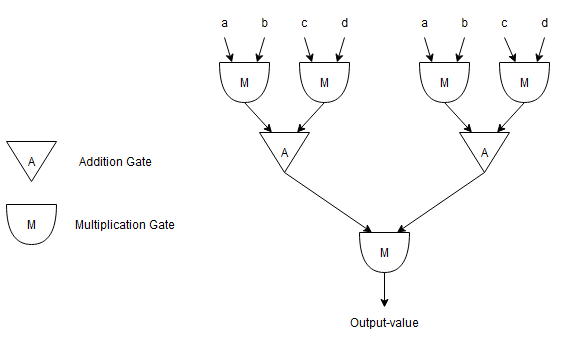
\includegraphics[width=0.7\textwidth, height=5.5cm]{arithmetic_circuit_EXAMPLE.png}
  \centering
  \label{fig:circuit_example}
\end{SCfigure}

\subsection{Notation and other terminology} 
\label{sect:prelims_other}

The following table holds useful notation and their definitions. 
The terms and notation are given on the left, and their definitions on the
right.
\amnote{The \texttt{longtable} seems useful here}

\begin{tabularx}{\textwidth} { 
  %| 
  X %|
  X %| 
  }
 \hline
 $k$-multilinear monomial & a multilinear monomial that has a degree of $k$ \\
 \hline
 sum of monomials form & an expression for a polynomial $P(X)$ where there are no 
 polynomial multiplications present, i.e., the expression consists of only additions between monomials \\
 \hline
 $\mathcal{O}$* & hides factors polynomial to the input size, e.g., \bigO{n^3k^n} = \bigOstar{k^n} \\
 \hline
 FPT & A class of \emph{fixed parameter tractable} problems, i.e., parameterized problems that 
 can be solved in polynomial time if the parameter is fixed \\
 \hline
 $poly(n)$ & a polynomial function in $n$, e.g., $an^4 + bn + c$ \\
 \hline
 Deterministic algorithm & Given a fixed input, a \emph{deterministic} algorithm always gives the same output \\
 \hline
 Randomized algorithm & A \emph{randomized} algorithm relies on pseudorandom 
 functions, and may not produce the same outputs for a fixed input\\
 \hline
 Schwartz-Zippel lemma & TODO: give here or in the context? \\
 \hline
 term & def \\
 \hline
\end{tabularx}
\amnote{Drop example for polynomial in $n$}
\amnote{No need to define deterministic / randomized algorithm}
\amnote{S-Z lemma in text seems better}
\amnote{$k$-multilinear monomial is better defined before in context}

Schwartz-Zippel ref:

J. T. Schwartz, “Fast probabilistic algorithms for verification of
polynomial identities,” Journal of the ACM, vol. 27, no. 4, pp. 701–717,
1980.



\clearpage
\section{General multilinear monomial detection}
\label{sect:general_mld}

The detection of multilinear monomials in a multivariate polynomial is a fundamental problem, 
since many important problems can be reduced to it, 
as seen in Section \ref{sect:related_problems}. 
Therefore, any progress in general multilinear monomial detection implies 
faster algorithms for the problems mentioned in Section \ref{sect:related_problems}.

In this section, 
we discuss the algebraic ideas by \citeauthor{KouWil09} \cite{Koutis08, Williams09, KouWil09} 
for the $k$-multilinear monomial detection. 
In Section \ref{sect:algebraic_fingerprinting}, 
we dive into the technique of \emph{algebraic fingerprinting}, and 
see the ideas and implementations of \citeauthor{KouWil09}. 
In Section \ref{sect:complexity} we briefly discuss the time and space complexity 
of the general algebraic framework given by algebraic fingerprinting. 
Finally, Section \ref{sect:limits} discusses the limits of algebraic fingerprinting.

As a prelude for the following sections, recall the relevant problem definition: 
\begin{problem}
  \problemtitle{$k$-\textsc{multilinear monomial detection}}
  \probleminput{A commutative arithmetic circuit $A$ representing a polynomial $P(X)$.}
  \problemquestion{Does the polynomial $P(X)$ extended as a sum of monomials 
  contain a multilinear monomial of degree $k$?}
\end{problem}

\subsection{Algebraic fingerprinting}
\label{sect:algebraic_fingerprinting}

In Section \ref{sect:problem_definition}, we discussed non-algebraic methods 
for approaching $k$-multilinear monomial detection. In particular, we mention
an interesting idea of discarding squared variables when dynamically 
computing the circuit. From this, we build towards algebraic fingerprinting. 

This idea of discarding squared variables as soon as they are formed in $A$ 
can be expressed mathematically: any squared variable should be identical to
zero. 
\begin{equation}
  \label{eq:squared_to_zero}
\forall x \in X: x^2 = \mathbf{0}
\end{equation}
This implies that any non-multilinear monomial in $X$ will evaluate to zero in $P(X)$, since 
any non-multilinear monomial $q$, assuming commutativity, can be written as $x^2q'$ 
for some $x \in X$, and $x^2q' = \mathbf{0}q' = \mathbf{0}$ over any algebra. 
Therefore, $P(X)$ will identically evaluate to zero if there are no multilinear monomials, 
i.e., there exist no solutions to the original problem.

This is the basis of algebraic multilinear monomial detection introduced by 
\citeauthor{Koutis08} \cite{Koutis08}, 
or later referred to as \emph{algebraic fingerprinting} \cite{KouWil15}: 
we evaluate $P(X)$ over some algebraic structure $\mathbf{G}$, 
and detect a multilinear monomial from 
the value returned by this evaluation. Ideally, with any 
evaluation of $P(X)$ at any $Z \subset \mathbf{G}, \abs{Z} = \abs{X}$ 
where $w \neq \mathbf{0}$, 
\begin{equation}
  \label{eq:polynomial_identity}
  P(Z) =
    \begin{cases}
      \mathbf{0} & \text{if no multilinear monomials exist}\\
      w & \text{otherwise}\\
    \end{cases}       
\end{equation}

In the following subsections, we specify an appropriate algebraic structure such that 
(\ref{eq:polynomial_identity}) is met, as well as some requirements for efficiency. 
Then, we discuss the works of \citeauthor{Koutis08} 
and \citeauthor{Williams09} \cite{Koutis08, Williams09}, 
and see how these specifications were implemented.

This thesis refers to the general framework provided 
by this algebraic technique for parameterized problems \cite{KouWil09, KouWil15} as 
algebraic fingerprinting. However, algebraic fingerprinting can also 
be used to refer specifically to the idea behind solving a problem 
with multilinear monomials canceling out due to characteristic,  
which is discussed in Section \ref{sect:fingerprints}.

\subsubsection{Specifications for the algebraic structure}
\label{sect:algebra_specs}

We have arrived at an important task for multilinear monomial detection: 
find an appropriate algebraic structure $\mathbf{G}$ for 
the evaluation of $P$ over $\mathbf{G}$ to meet 
(\ref{eq:squared_to_zero}) and thus the first equality in (\ref{eq:polynomial_identity}). 
We specify for commutative algebraic structures such as 
commutative rings for multilinear monomial detection; 
$\mathbf{G}$ should have commutative multiplication in order for (\ref{eq:squared_to_zero}) 
to be effective. The ordering of indeterminates in monomials is generally unknown, 
since the specific algebrization into multilinear monomial detection 
is abstracted away. %Specifying for commutativity also makes it significantly 
%easier to algebrize problems into arithmetic circuits. 

For the second equality in (\ref{eq:polynomial_identity}), it is necessary that multilinear 
monomials in $P(X)$ are not identical to $\mathbf{0}$ over $\mathbf{G}$. 
More specifically, 
$w$ should not be identical to $\mathbf{0}$. 
Thus, it must be that $k \leq \abs{\mathbf{G}}$, where $k$ is the degree of the monomials. 
Although this is not enough to ensure that $w \neq \mathbf{0}$ (as seen in the following section), 
we leave the issue for now.

These are the necessary specifications for $\mathbf{G}$ for algebraic multilinear monomial detection. 
However, this algebraic detection must be efficient for it to be useful. 
Therefore, further requirements are necessary: (a) the binary operations of $\mathbf{G}$ 
must be efficiently computable %fast
for a fast evaluation of $P(X)$, and (b) multilinear monomials in $P(X)$ must 
survive the evaluation of $P$ under an assignment $\gamma \colon X \to \mathbf{G}$ 
with a constant probability. We reason the 
sudden appearance of \emph{survivability} and probabilities soon.

Recall from Section \ref{sect:problem_definition} 
that with color coding, multilinear monomials can be detected with a 
randomized algorithm in \bigOstar{(2e)^k} time. Thus for (a), we may specify for 
an evaluation of $P(X)$ to take \bigOstar{2^k} time. The polynomial $P(X)$ 
will have at most $2^k$ multilinear monomials. Therefore, 
it is necessary that the binary operations 
of $\mathbf{G}$ take polynomial time.

With (b), recall that multilinear monomials 
survive color coding with probability $e^{-k}$. 
With algebraic fingerprinting, although not identical to zero, a multilinear monomial in $P(X)$ 
can still evaluate to $\mathbf{0} \in \mathbf{G}$ under some assignment $\gamma \colon X \to \mathbf{G}$. 
However, if we specify for a constant 
probability of survival under random $\gamma$, we can reliably decide whether a multilinear monomial exists 
by evaluating $P(X)$ in $\mathbf{G}$ over a constant number of 
randomized assignments $X \to \mathbf{G}$. Relating to color coding, 
this would essentially remove the 
$e^k$ factor in \bigOstar{(2e)^k}.

To restate, we now have to find such a commutative ring $\mathbf{G}$ that 
meets the following specifications: 
\begin{itemize}
  \item $\forall g \in \mathbf{G} \colon g^2 = \mathbf{0}$
  \item Operating over $\mathbf{G}$ should be fast, i.e., evaluating 
  $P(X)$ should take \bigOstar{2^k} time.
  \item Multilinear monomials should evaluate to non-zero
  through a random assignment 
  $\gamma \colon X \to \mathbf{G}$ with a reasonable constant probability.
\end{itemize}

In the work that introduced 
this algebraic fingerprinting technique \cite{Koutis08}, 
\citeauthor{Koutis08} used the group algebra $\Z_2[\Z_2^k]$. 
\citeauthor{Williams09} developed the technique further, 
generalizing the algebra to $GF(2^{l})[\Z_2^k]$ \cite{Williams09}. 
Next, we look at these group algebras of $\Z_2^k$ for $\mathbf{G}$. 

\subsubsection{Using group algebras of $\Z_2^k$}

The multiplicative group $\Z_2^k$ consists of $k$-dimensional \{0,1\}-vectors 
with the binary operation defined as component-wise addition modulo 2. 
For example with $k = 3$, 
\[
  \begin{bmatrix} 0 \\ 0 \\ 1 \end{bmatrix} \cdot 
  \begin{bmatrix} 0 \\ 0 \\ 1 \end{bmatrix} =
  \begin{bmatrix} 0 \\ 0 \\ 0 \end{bmatrix} = \mathbf{0} \in \Z_2^3.
\]
Observe that in general, every element in $\Z_2^k$ is its own inverse:
\begin{equation}
  \label{eq:Z_2^k has char 2}
  \forall z \in \Z_2^k \colon z^2 = \mathbf{0}.
\end{equation}
Recall that the elements of a
\amnote*{Actually an algebra over a field?}{group algebra}
$\mathbf{F}[\Z_2^k]$ are linear combinations of the form 
\[
  \displaystyle \sum_{v \in \Z_2^k}a_v v,
\]
where $a_v \in \mathbf{F}$. From here on, we note the identity of $\Z_2^k$ as $v_0$, additive and 
multiplicative identities of $\mathbf{F}$ as $\mathbf{0}_F$ and $\mathbf{1}_F$, respectively, and 
use $\mathbf{0}$ and $\mathbf{1}$ for the identities of 
$\mathbf{F}[\Z_2^k]$. Recall that $\mathbf{1} = v_0$, and
$\mathbf{0}$ corresponds to the element $\sum_{v \in \Z_2^k}a_v v$, where $a_v =
\mathbf{0}_F$. Note that + represents addition over $\mathbf{F}[\Z_2^k]$ and not 
addition over $\Z_2^k$ which is a multiplicative group.
%\amnote{So if we represent the elements of $\mathbf{F}[\Z_2^k]$ as vectors, we
%get vectors with $2^k$ entries}

In his introductory work for this technique \cite{Koutis08}, 
\citeauthor{Koutis08} assigned $X$ 
to elements of the form $(v_0 + v_i) \in \mathbf{F}[\Z_2^k]$, 
such that for every $x_i \in X$, a random $v_i \in \Z_2^k$ is independently and uniformly 
picked for the assignment 
$\gamma(x_i) = v_0 + v_i$. %{$x_i \to (v_0 + v_i)$.} 
We note the assigned values as $\overbar{X}$, and the resulting element  
from the polynomial evaluation 
as $P(\overbar{X}) \in \mathbf{F}[\Z_2^k]$. 
\citeauthor{Koutis08} observed that 
due to (\ref{eq:Z_2^k has char 2}), for all $v \in \Z_2^k$ and $(v_0 + v) \in \mathbf{F}[\Z_2^k]$, 
\[
  (v_0 + v)^2 = v_0^2 + v_0v + vv_0 + v^2 = v_0 + v + v + v_0 = 2v_0 + 2v.
\]
This implies that if we pick a field with characteristic 2 for $\mathbf{F}$, 
$\forall v_i \in \Z_2^k \colon (v_0 + v_i)^2 = \mathbf{0}$. Thus, 
non-multilinear monomials in $P(X)$ vanish in $P(\overbar{X})$, and the 
first equation in (\ref{eq:polynomial_identity}) 
will hold.

However, if $\mathbf{F}$ has characteristic 2, the second equation of (\ref{eq:polynomial_identity}) 
does not necessarily hold, and it may be that $w = \mathbf{0}$. Multilinear monomials may 
cancel each other out in $\mathbf{F}[Z_2^k]$, since they may have even leading 
coefficients in $P(X)$. Next, we see how \citeauthor{Koutis08} approached this problem.

%Such $\mathbf{G}$ is given in \cite{Koutis08}, where \citeauthor{Koutis08} uses the group $\Z_2^k$ 
%and a known \cite{Terras99} 
%isomorphic mapping $\rho \colon \Z_2^k \to M^{2^k \times 2^k}$, where $M^{d \times d}$ is a 
%\amnote*{Any group? Specific one?}{$d$-dimensional matrix group with matrix multiplication.}
% Note that for (\ref{eq:squared_to_zero}), 
%\[
%\forall a \in \Z_2^k \setminus \{\mathbf{0}\}, i \in [2^k]: \rho(a)_{i,i} = 0\]and \[
%\rho(\mathbf{0}) = \mathbf{0}.
%\]
\subsubsection{Fingerprints to prevent unwanted cancelation}
\label{sect:fingerprints}

Indeed, if we take the $k$-3D matching instance from Section \ref{sect:algebrization}, 
we notice that the multilinear monomials in $P_2$ have even coefficients, and thus 
would cancel out in $\mathbf{F}[Z_2^k]$ due to characteristic.
\begin{multline*}
  P_2 = (a_1b_1c_1 + a_1b_2c_2 + a_2b_2c_3)^2  \\
  = a_1^2b_1^2c_1^2 + a_1^2b_2^2c_2^2 + a_2^2b_2^2c_3^2 + %\allowbreak
  2a_1^2b_1b_2c_1c_2 + 2a_1a_2b_1b_2c_1c_3 + 2 a_1a_2b_2^2c_2c_3. 
\end{multline*}
In general, when $k$ is even, multilinear monomials will have even coefficients. 

To tackle this issue, one idea is to add auxiliary indeterminates, 
called \emph{fingerprints} \cite{KouWil15}, to the monomials 
in order to make them unique. For example, let
\amnote*{Actually $S = \{ s_1,\dots,s_6 \}$?}{
$S = \{s_1, s_2, \ldots\}$ 
be the set of an appropriate number of fingerprints 
}
and augment them to $P_k$ as follows: 
\amnote{Use \texttt{\textbackslash align}}
\begin{multline*}
  P'_2 = (s_1a_1b_1c_1 + s_2a_1b_2c_2 + s_3a_2b_2c_3)(s_4a_1b_1c_1 + s_5a_1b_2c_2 + s_6a_2b_2c_3) \\
  = s_1s_4a_1^2b_1^2c_1^2 + s_2s_5a_1^2b_2^2c_2^2 + s_3s_6a_2^2b_2^2c_3^2 + \\
  s_1s_5a_1^2b_1b_2c_1c_2 + s_2s_4a_1^2b_1b_2c_1c_2 + s_1s_6a_1a_2b_1b_2c_1c_3 + \\
  s_3s_4a_1a_2b_1b_2c_1c_3 + s_2s_6a_1a_2b_2^2c_2c_3 + s_3s_5a_1a_2b_2^2c_2c_3. 
\end{multline*}

\amnote*[inline,nomargin]{Now the multilinear monomial $a_1a_2b_1b_2c_1c_3$ only
cancels itself out in $\rho(P'_2)$ ($P'_2(Z)$? unsure about notation) if
$\rho(s_1)\rho(s_6) = \rho(s_3)\rho(s_4)$ under the assignment $\rho$ ....
We can control depending on how the $\rho(s_i)$ are chosen...}{
Then, the multilinear monomial detection algorithm 
could assign every $a \in X \cup S$ to $\mathbf{F}[\Z_2^k]$. 
}
With this, non-multilinear monomials will still vanish, but multilinear monomials 
will not identically cancel each other out when $k$ is even. 

However, introducing new indeterminates raises the degree of multilinear
monomials. 
\amnote*{??}{
Therefore, it increases the probability that indeterminates in a multilinear monomial are 
assigned the same value from $\mathbf{F}[Z_2^k]$, which results in the 
multilinear monomial evaluating to zero with higher probability. 
}
Counteractively raising the dimension of $\Z_2^k$, however, would  
exponentially slow down matrix multiplications which prove to be %matrix mulitplication has a time complexity of \bigO{n^2.31788} \cite{DuanZhouWu22}. 
important for efficiency in algebraic fingerprinting (see Section \ref{sect:complexity}).

\citeauthor{Koutis08} approached this problem by assigning fingerprints to elements 
from a different algebraic structure: he used $S \to \Z_2$ and set 
$\mathbf{F} = \Z_2$ \cite{Koutis08}. In this sense, 
fingerprints are defined to be auxiliary coefficients instead of auxiliary indeterminates. 
Note that $\Z_2$ has characteristic 2. With this, 
\citeauthor{Koutis08} essentially assigns multilinear monomials a coefficient 
randomly from $\{\mathbf{0}_F, \mathbf{1}_F\}$. The idea is that a multilinear monomial, 
assigned with the fingerprint $\mathbf{1}_F$,  
survives the cancelation due to characteristic if the canceling pair is assigned $\mathbf{0}_F$. 
With randomized assignments $S \to \Z_2$, 
there is a constant \amnote[inline,nomargin]{positive} probability that a multilinear 
monomial will have an odd coefficient, and thus survive the assignment \cite{Koutis08}.

In practice, fingerprints can be implemented 
into the algebrization as follows (see also Figure \ref{fig:circuit_fingerprints}): 
for every multiplication gate $G_i$ feeding from the
\amnote*{inputs}{terminals} in the arithmetic circuit $A$ for $P(X)$, 
pick a unique $s_i \in S$. Insert a new multiplication gate $\overbar{G_i}$ that takes 
as input $s_i$ and the output of $G_i$. The output of $\overbar{G_i}$ feeds to the 
gates that read the output of $G_i$. We note the new polynomial represented by this circuit 
as $P'(X, S)$. Note that here, 
\citeauthor{Koutis08} picked random elements from $\Z_2$ for $s_i$.

\begin{figure}[h]
  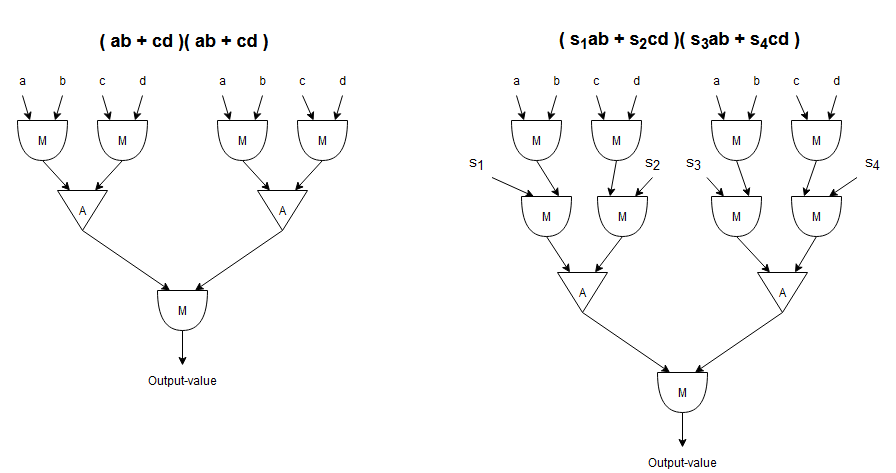
\includegraphics[width=\textwidth, height=7cm]{arithmetic_circuit_FINGERPRINTS.png}
  \centering
  \caption{A fingerprinted circuit for evaluating $(ab+cd)^2$. 
  Note the added terminals on the right circuit.}
  \label{fig:circuit_fingerprints}
\end{figure}

\subsubsection{Polynomial identity testing}

From another perspective, we may look at algebraic fingerprinting as \emph{polynomial identity testing}. 
That is, we compute $P'(X, S)$ over assignments $X \to \mathbf{F}[\Z_2^k]$ into $P'(\overbar{X}, S)$, i.e., 
compute until the gates $\overbar{G_i}$. 
Imagine we stop here in the circuit before assigning the fingerprints $S$  
and continuing with the multiplication. 
Currently, we may see $P'(\overbar{X}, S) \in \mathbf{K}[S]$ as a polynomial 
with indeterminates from $S$ and coefficients from $\mathbf{K} = \mathbf{F}[\Z_2^k]$. 
In a sense, we switch the roles of coefficients and indeterminates in $P'(X, S)$ 
to find a new polynomial $Q(S) \in \mathbf{K}[S]$. 

Now, deciding whether a multilinear monomial exists in $P(X)$ is essentially given by 
whether the polynomial $P'(\overbar{X}, S) \in \mathbf{K}[S]$ is identical to $\mathbf{0}$, 
i.e., with $\Phi$ representing the family of mappings $S \to \mathbf{F}$ 
and $\phi(S)$ representing the assigned values of $S$ with $\phi$,  
\[
  \forall \phi \in \Phi %, \overbar{S} = \{\phi(s) \: | \: s \in S\} 
  \colon P'(\overbar{X}, \phi(S)) = \mathbf{0}.
\]
Therefore, we formulate algebraic fingerprinting as polynomial identity testing, i.e., 
we test wheter $P'(\overbar{X}, S) \in \mathbf{K}[S]$ is identical to $\mathbf{0}$.

\begin{problem}
  \problemtitle{\textsc{Polynomial identity testing}}
  \probleminput{An arithmetic circuit $C$ that computes the polynomial $Q(S)$.}
  \problemquestion{Is $Q(S)$ identical to the zero polynomial?}
\end{problem}

We frame $P'(\overbar{X}, S)$ as $Q(S) \in \mathbf{K}[S]$. 
Here, it is necessary to test whether $Q(S)$ is identical to \emph{zero modulo 2}, 
since we used characteristic 2 to eliminate 
the underlying non-multilinear monomials in $P'(\overbar{X}, S)$.

Thus, multilinear monomial detection is reduced via algebraic fingerprinting 
to polynomial identity testing. A multilinear monomial is detected if 
$Q(f) \neq \mathbf{0}_F \in \mathbf{F}$, where $Q(f)$ 
represents evaluation under an assignment $S \to \mathbf{F}$, 
with any field $\mathbf{F}$ of characteristic 2. 
We note the family of assignments $S \to \mathbf{F}$ as $\Phi$.

Assume multilinear monomials exist in $P(X)$. 
\citeauthor{Koutis08} \amnote*[inline,nomargin]{managed}{achieved} to detect a multilinear monomial 
with \amnote[inline,nomargin]{(a)} probability $(1/4 + 1/{4k})$ by testing whether 
$Q(S) = \mathbf{0}$ over the field $\mathbf{F} = \Z_2$  
with randomized assignments $S \to \Z_2$ \cite{Koutis08}. 
\citeauthor{Williams09} developed the technique of algebraic fingerprinting 
further by observing that due to the Schwartz-Zippel lemma, %(see \cref{sect:prelims}), 
if we raise the order of the field $\mathbf{F}$ 
such that the number of different assignments in $\Phi$ is much larger than 
the number of assignments $\phi \in \Phi$ that have $Q(\phi(S)) = \mathbf{0}_F$, 
$Q(\delta(S)) \neq \mathbf{0}_F$ with a high probability over some $\delta \in \Phi$ 
\cite{Williams09}. 

Of course, $\mathbf{F}$ must have characteristic 2. For this, \citeauthor{Williams09} 
used the field $GF(2^{l})$ with $l \in \N$. \cite{Williams09}. By Schwartz-Zippel lemma, $Q(S)$ 
evaluates to $\mathbf{0}_F$ over a random assignment $S \to GF(2^{3+log_2k})$ with probability 
at most $k/\abs{\mathbf{F}}$ \cite{Williams09}. For example with $k$-path, 
\amnote{Use \texttt{\textbackslash log}}
\citeauthor{Williams09} used $l = 3+ log_2k$, 
which sets the probability of a false-negative evaluation 
to at most $k/\abs{\mathbf{F}} = 1/2^3$. 
For the $k$-path problem, \citeauthor{Koutis08} 
gave a randomized \bigOstar{2^{3k/2}} time algorithm \cite{Koutis08}, 
and \citeauthor{Williams09} developed this into a randomized \bigOstar{2^k} 
time algorithm \cite{Williams09} with the ideas discussed here.

In the following section, we briefly touch on the complexities of the 
algebras given here. 

\subsection{Time and space complexity}
\label{sect:complexity}

In the previous section, we discussed the specifications 
for an algebraic stucture to implement algebraic fingerprinting. 
For an appropriate algebra, we found $GF(2^{l})[Z_2^k]$. 
However, we did not discuss the costs related 
to this algebra. In this section, we briefly discuss the time and space complexity 
of algebraic fingerprinting.

Define the evaluation of $P'(X, S)$ at any $X$ and $S$ to take $g(n)$ number of  
arithmetic operations, where $n = \abs{X}$. In general, 
detecting $k$-degree multilinear monomials in $P(X)$ takes 
\bigOstar{2^kg} time and \bigO{poly(n,k)} space \cite{Williams09}.

Actually, the complexities given by \citeauthor{Koutis08} \cite{Koutis08} and 
\citeauthor{Williams09} \cite{Williams09} did not directly come from 
$\Z_2[Z_2^k]$ or $GF(2^{l})[Z_2^k]$. 
To make the complexity claims in \cite{Koutis08}, 
\citeauthor{Koutis08} used a well-known \cite{Terras99} isomorphism 
$\kappa \colon \Z[\Z_2^k] \to \mathcal{M}$, where $\mathcal{M} = \mathbf{M}^{2^k \times 2^k}$ 
is an algebra of special permutation matrices with binary entries. To translate $\Z[\Z_2^k]$ to 
$\Z_2[\Z_2^k]$, it is enough to take the modulo 2 of the coefficients $a_v$ in 
the elements of $\Z[\Z_2^k]$: 
\amnote{No need for displaystyle}
\[
  %\displaystyle
  \sum_{v \in \Z_2^k}a_v v \in \Z[\Z_2^k] \implies 
  %\displaystyle \sum_{v \in \Z_2^k}(a_v \: mod \: 2) v \in \Z_2[\Z_2^k]
  \displaystyle \sum_{v \in \Z_2^k}(a_v \bmod 2) v \in \Z_2[\Z_2^k]
\]
\amnote{Use \texttt{\textbackslash bmod}}

%Thus, if we assign $S$ to $\Z$, it is enough to consider the parity of 
%the coefficient of $v_0 \in \Z_2^k$ in $P_S(\overbar{X})$ \cite{Koutis08}. 
Since \citeauthor{Koutis08} 
used an isomorphism, all the ideas given in 
Section \ref{sect:algebraic_fingerprinting} still hold for 
detecting multilinear monomials. That is, 
the given implementation for (\ref{eq:polynomial_identity}) is valid through $\kappa$.

\omnote*{Maybe don't go further than this}{Using these matrices, }
\amnote{I would rather expand in Sect. 5 than here}
\citeauthor{Koutis08} \cite{Koutis08} detected $k$-multilinear monomials 
by computing the \omnote*{add to prelims?}{trace} of the matrix resulting 
from the evaluation of $P_S(X)$ over $\mathcal{M}$. The trace can be computed 
in time \bigO{2^k(nk+t)} and space \bigO{nk+s}, where $t$ and $s$ are the time 
and space complexity of the $g(n)$ arithmetic operations, respectively. 

For $GF(2^{l})[Z_2^k]$, the same ideas are used, though we omit 
further discussion into this for the sake of brevity. 
Thus, we have a general 
\bigOstar{2^kg} time and \bigO{poly(n,k)} space algorithm for detecting 
$k$-degree multilinear monomials in $P(X)$, where $g$ is the number of gates in the 
arithmetic circuit for $P(X)$ and $n = \abs{X}$ \cite{KouWil09}.

It is important to note here that this complexity is for $k$-degree 
multilinear monomial detection. Whether a parameterized problem with a parameter 
$k$ receives an \bigOstar{2^k} time algorithm, is determined by the algebrization 
of said parameterized problem. 
For example for $k$-path, algebraic fingerprinting gives an \bigOstar{2^k} 
time algorithm \cite{Williams09}. 
For $k$-3D-matching however, as given in Section \ref{sect:algebrization}, 
algebraic fingerprinting gives an \bigOstar{2^{3k}} algorithm, since 
$k$-3D-matching reduces into $3k$-degree multilinear monomial detection.


\subsection{Limits of algebraic fingerprinting}
\label{sect:limits}

In this section, we discuss some limiting factors to the general 
algebraic framework given by 
algebraic fingerprinting for parameterized problems. First, 
we discuss the lower bound for the runtime. Then, we discuss 
the difficulties for derandomization. Finally, we touch on
\amnote[inline,nomargin]{the issue of}
finding a solution for the underlying combinatorial problem 
whereas algebraic fingerprinting only detects
\amnote*[inline,nomargin]{that one exists}{one}.

\subsubsection{Algebraic optimization}
\label{sect:algebra_is_optimal}

In Section \ref{sect:complexity}, it was established that $k$-multilinear monomials 
in $P(X)$ are detected with 
algebraic fingerprinting in \bigOstar{2^kg} time, where 
$g$ is the number of gates in the arithmetic circuit for $P(X)$ \cite{Williams09}. 
This time was achieved by evaluating the circuit over matrix 
representations of the algebra $GF(2^l)[\Z_2^k]$.

%Furthermore, 
\citeauthor{KouWil09} showed that this particular algebra is nearly optimal 
for time complexity \cite{KouWil09}: there is no significantly faster algebra that 
is appropriate for the general $k$-multilinear monomial detection. 
The authors proved that if any commutative algebra $\mathcal{G}$ is 
used for detecting $k$-multilinear monomials, 
the lengths of elements in $\mathcal{G}$ must be \bigOmega{2^k/k}.

Thus for the general $k$-multilinear monomial detection, we may say 
that algebraic fingerprinting is in some sense optimized. 
However, 
ideas from algebraic fingerprints can be utilized for faster algorithms for 
specific $k$-multilinear monomial detection instances (see Section \ref{sect:improvements}).

\subsubsection{Derandomization}
\label{sect:derandomization}

Algebraic fingerprinting gives a randomized algorithm for $k$-multilinear monomial detection. 
The derandomization of the general framework seems hard, since algebraic fingerprinting 
uses the fact that polynomial identity testing can be solved in polynomial time with 
a randomized algorithm \cite{Williams09}.

If algebraic fingerprinting can be derandomized 
in polynomial time, it implies that polynomial identity testing can be solved with a 
polynomial time deterministic algorithm. This would imply strong circuit lower bounds 
TODO: this is apparently significant

\begin{anamnote}[nomargin]
  If this gets into too hairy complexity theory territory, just say it would
  imply \enquote{surprising results} in complexity theory.
  People usually can imagine what that means...
\end{anamnote}

\subsubsection{Finding the solution}
\label{sect:finding_the_solution}

In many instances of multilinear monomial detection, 
a solution to the underlying problem can be directly found 
from the multilinear monomials by
\amnote*{reverse-engineering}{reverse engineering} the algebrization. 
However in algebraic fingerprinting, we do not have this information on the monomials: 
when we assign the variables values and evaluate the polynomial, we may only detect the 
presence of a solution. As such, algebraic fingerprinting applies to decision algorithms.

However, finding a solution when its presence is detected
\amnote*{??}{seems easy}. 
Moreover, since most of the problems in Section \ref{sect:related_problems} 
have search problems in FPT, a solution is found in polynomial time when its 
existence is detected.

For example, in \cite{Koutis08}, 
\cite{Koutis08} gives an algorithm that detects a $k$-path, and shows that a 
$k$-path can be found by \bigOstar{n+min(k^2, m)} applications of the given
algorithm. 
\amnote{What are $n$ and $m$ here? (I can imagine, but some other reader probably won't)}
In general for subgraph problems, we may find a solution by calling the decision 
algorithm a polynomial number of times for different subgraphs of the original input graph.

\amnote{dropped clearpage}
%\clearpage
\section{Improving from algebraic fingerprinting}
\label{sect:improvements}

As mentioned in Section \ref{sect:algebra_is_optimal}, 
algebraic fingerprinting as a framework %proposed by 
%\citeauthor{Koutis08} and \citeauthor{Williams09} \cite{Williams09, KouWil09, KouWil15} 
for $k$-multilinear monomial detection has a lower bound of \bigOmega{2^k}. 
However, this framework is very generic since it 
approaches the abstracted multilinear monomial detection without 
utilizing the combinatorial properties specific to the underlying problem. 
The idea of adding auxiliary fingerprint variables in the algebrization, though, 
has potential for these properties.

Indeed, faster algorithms for specific combinatorial problems 
have been found by designing new algebrizations with techniques 
similar to algebraic fingerprinting, where the fingerprints are designed to make use of 
the underlying combinatorial properties. In Section \ref{sect:cancel_nonsolutions}, 
we see how \citeauthor{Björklund14} \cite{Björklund14} 
exploited the cancelation due to characteristic to cancel non-solution monomials 
by clever design of fingerprints. 

Section \ref{sect:other_improvements} briefly overviews other ideas or 
improvements in utilizing the general framework of algebraic fingerprints.

\subsection{Fingerprinting for cancelation of non-solutions}
\label{sect:cancel_nonsolutions}

TODO: go over Björklund et al. for k-path or Hamiltonicity, managed to design
fingerprints such that non-solutions cancel

\begin{anamnote}[nomargin]{}
  We already have plenty of content.
  Either cut some content before or keep things here very brief!
\end{anamnote}

In the algebraic framework by \citeauthor{Koutis08} and \citeauthor{Williams09}, 
fingerprints prevent the cancelation of multilinear monomials. 
Attacking the Hamiltonian path problem, however, \citeauthor{Björklund14} 
designed fingerprints such that non-multilinear monomials, i.e. non-solution terms, 
cancel due to characteristic, while the multilinear terms 
remain with constant probability \cite{Björklund14}. This resulted in the current 
fastest algorithm for undirected Hamiltonicity, running in \bigOstar{2^n} time.

Before discussing the algebrization and the fingerprints, 
we define the Hamiltonian path problem.

\begin{problem}
  \problemtitle{\textsc{Hamiltonian path (Hamiltonicity)}}
  \probleminput{A directed graph $G = (V,E)$.}
  \problemquestion{Does $G$ contain a simple path that visits every vertex?}
\end{problem}

\omnote*{Probably really brief}{TODO: give the algebrization and/or show how it works}

\subsection{Other research in improving algebraic fingerprinting}
\label{sect:other_improvements}

- constrained multilinear detection (weighted problems?), temporal graphs

- deterministic multilinear detection (partial differentials of polynomials)

As briefly discussed in /Cref{sect:derandomization}, algebraic fingerprinting 
gives randomized algorithms, and the derandomization is hard. 

- distributed multilinear detection (MIDAS-paper)
%Furthermore, the evaluation of the polynomial in the algebraic fingerprinting framework is done sequentially. 
%However, the matrix representations of the group algebras used in \cite{Williams09} 
%offer possibilities for parallelization.
%In \cref{sect:parallelization}, \amnote[inline,nomargin]{we discuss} the ideas of 
%\citeauthor{Midas19} behind the distributed multilinear monomial detection
%\cite{Midas19} \amnote*[inline,nomargin]{}{(are discussed)}.

%\clearpage
\section{Conclusion}
\label{sect:conclusion}

From Section \ref{sect:related_problems}, 
it can be seen  
that a fast algorithm for $k$-multilinear monomial detection gives a 
fast algorithm for many parameterized combinatorial problems. 
We found that algebraic fingerprinting solves this problem by 
evaluating the given multivariate polynomial over a specific algebra. 
Thus, we 
may say that algebraic fingerprinting gives a general framework for 
parameterized combinatorial problems. 

In Section \ref{sect:algebraic_fingerprinting}, we discussed the idea behind 
algebraic fingerprinting: generate a polynomial $P(X)$ from the algebrization of 
a combinatorial problem, and evaluate $P(X)$ over $GF(2^{l})[Z_2^k]$ with 
randomized assignments $X \to GF(2^{l})[Z_2^k]$ of form 
$x_i \to (v_0 + v_i)$, augmented with scalar multiplications 
by elements randomly chosen from $GF(2^{l}) \setminus \{\mathbf{0}\}$. 
This gives a randomized algorithm for 
$k$-multilinear monomial detection that runs in \bigOstar{2^k} time.

Moreover, as seen in Section \ref{sect:cancel_nonsolutions}, 
the technique of algebraic fingerprints can be utilized for even 
faster algorithms. In particular, a near fifty-year stagnation 
in improvements for the well-studied Hamiltonian path problem saw 
a significant development by \citeauthor{Björklund14} right after 
the novel algebraic technique \cite{Koutis08} saw publication.

TODO: conclude

\begin{anamnote}[nomargin]{}
  What about further work?
  What do people intend to work on in the near future?
\end{anamnote}